\documentclass{standalone}
\usepackage{tikz}
\usepackage{currfile}
\usepackage[mode=buildnew]{standalone}
\usetikzlibrary{spy}
\tikzset{
	mirror scope/.is family,
	mirror scope/angle/.store in=\mirrorangle,
	mirror scope/center/.store in=\mirrorcenter,
	mirror setup/.code={\tikzset{mirror scope/.cd,#1}},
	mirror scope/.style={mirror setup={#1},spy scope={
			rectangle,lens={rotate=\mirrorangle,yscale=-1,rotate=-1*\mirrorangle},size=80cm}},
}
\newcommand\mirror[1][]{\spy[overlay,#1] on (\mirrorcenter) in node at (\mirrorcenter)}

\begin{document}
	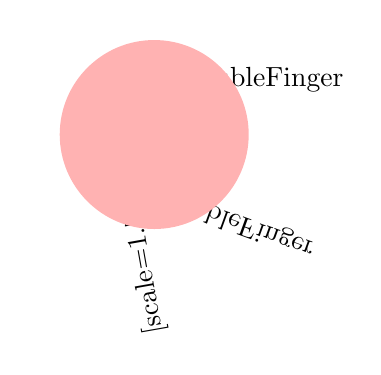
\begin{tikzpicture}
		\draw[white] (-3,-1) rectangle (0.5,0.65);	
		\node[draw=none,fill=none,rotate=100] at (-1.6,-2) {\includestandalone[scale=1.5]{\currfiledir finger}};
		\begin{scope}[mirror scope={center={-0.8,-0.8},angle=170}]
			\node[draw=none,fill=none] at (0,0) {\includestandalone{\currfiledir doubleFinger}};
			\mirror;
		\end{scope}
		\fill[red!30!white] (-1.4,-0.7) circle (1.2cm);
	\end{tikzpicture}
\end{document}
